%%%%%%%%%%%%%%%%%%%%%%%%%%%%%%%%%%%%%%%%%%%%%%%%%%%%%%%%%%%%%%%%%%%%%%
% How to use writeLaTeX: 
%
% You edit the source code here on the left, and the preview on the
% right shows you the result within a few seconds.
%
% Bookmark this page and share the URL with your co-authors. They can
% edit at the same time!
%
% You can upload figures, bibliographies, custom classes and
% styles using the files menu.
%
%%%%%%%%%%%%%%%%%%%%%%%%%%%%%%%%%%%%%%%%%%%%%%%%%%%%%%%%%%%%%%%%%%%%%%

\documentclass[12pt]{article}
\usepackage{titling}
\usepackage{graphicx}

\usepackage{sbc-template}
\usepackage{float}

\usepackage{graphicx,url}

%\usepackage[brazil]{babel}   
\usepackage[utf8]{inputenc}  

     
\sloppy


\begin{document}

% Capa personalizada
\begin{titlepage}
    \centering
    % Inserindo a imagem (logotipo da universidade)
    
\includegraphics[width=10cm]{logo_ateneu.png}  % Certifique-se de que o nome da imagem está correto
    \vspace{1cm}
    {\huge\bfseries Comunicação de Dados NP1 - Subjetiva \par}
    \vspace{1.5cm}
    {\Large Wellington Almeida Silva\par}
    \vspace{0.5cm}
    {\large Centro Universitário Uniateneu\par}
    \vspace{0.5cm}
    {\large \texttt{wellingtonsilva11@aluno.uniateneu.edu.br}\par}
    \vfill
    {\large \today\par}  % Data da capa
\end{titlepage}

\newpage  % Nova página para o conteúdo principal


\begin{abstract}
The article explores Power Line Communication (PLC) technology, which uses power lines to transmit data. It addresses the main challenges of this technology, such as echo, caused by discontinuities in the line, like impedance mismatches or faulty connections, leading to signal reflection and degrading its quality. Another challenge discussed is noise, generated by electrical devices like motors and appliances, and by external interference such as radio signals, which distort data transmission. Attenuation is also mentioned, referring to the loss of signal strength over the network, especially across long distances or through older wires.The article also compares parallel and serial transmission methods. Parallel transmission allows for the simultaneous sending of multiple bits, increasing speed over short distances, while serial transmission sends data one bit at a time, making it more efficient over long distances. Additionally, the communication modes in PLC systems are described, including simplex (one-way transmission), half-duplex (alternating bidirectional transmission), and full-duplex (simultaneous bidirectional transmission), highlighting their different applications according to the needs for speed and simultaneity. The article concludes by emphasizing how these modes affect the performance of PLC networks, especially in home automation and communication scenarios.
\end{abstract}
     
\begin{resumo} 
O artigo explora a tecnologia de Power Line Communication (PLC), que utiliza as linhas de energia elétrica para transmitir dados. Ele aborda os principais desafios dessa tecnologia, como o eco, que é causado por descontinuidades na linha, como mudanças de impedância ou conexões mal feitas, levando à reflexão do sinal e prejudicando sua qualidade. Outro desafio discutido é o ruído, gerado por dispositivos elétricos, como motores e eletrodomésticos, e por interferências externas, como sinais de rádio, que distorcem a transmissão de dados. A atenuação é também mencionada, referindo-se à perda de intensidade do sinal ao longo da rede, especialmente em distâncias maiores ou em fios antigos. O artigo também compara os métodos de transmissão paralela e transmissão em série. A transmissão paralela permite o envio simultâneo de vários bits, o que aumenta a velocidade em curtas distâncias, enquanto a transmissão em série envia os dados um bit de cada vez, sendo mais eficiente para longas distâncias. Além disso, são descritos os modos de operação da comunicação em sistemas PLC, como o simplex (transmissão em uma única direção), half-duplex (transmissão bidirecional alternada) e full-duplex (transmissão bidirecional simultânea), destacando suas diferentes aplicações de acordo com as necessidades de velocidade e simultaneidade. O artigo conclui ressaltando como esses modos influenciam o desempenho das redes PLC, especialmente em cenários de automação residencial e comunicação.
\end{resumo}

\tableofcontents

\section{O que é uma PLC?} \label{sec:firstpage}

PLC (Power Line Communication) é uma tecnologia que permite a transmissão de dados através da rede elétrica. Ela utiliza a infraestrutura existente de cabos elétricos para transportar sinais de comunicação, ao mesmo tempo em que transmite eletricidade. PLC pode ser usada tanto para comunicação de dados de baixa velocidade, como em sistemas de automação, quanto para transmissões de internet em alta velocidade. A técnica de transmissão de dados via rede elétrica, apareceu pela primeira vez na década de 50, conhecida como RPC (Ripple Control), utilizando baixas frequências entre 100 e 900Hz, e potências de transmissão elevadas. Esse tipo de transmissão de dados perdeu relevância por volta dos anos 2000 com o avanço de tecnologias mais eficientes, como a fibra ótica, Wi-Fi e Ethernet, que oferecem maior largura de banda, confiabilidade e menor interferência. \cite{lopes2021}

Segundo \cite{devmedia}, "Primeiro os dados chegam nos acopladores, que podem ser capacitivos (injetam dados através de contado direto com a linha de energia elétrica) ou indutivos (injetam sinais por indução), o Master PLC ou 'head end' da rede, fica instalado próximo ao transformador e tem a função de gerenciar e rotear informações aos repetidores. Os repetidores regeneram e reinjetam o sinal PLC para a rede elétrica doméstica e por fim, o modem é conectado à tomada de energia da rede e, além de ser alimentado, ele recebe o sinal PLC através de uma tomada simples. O modem PLC normalmente possuía interfaces de comunicação RJ45 para ethernet, USB e RJ11 para telefones." 

\begin{figure}[H]
    \centering
    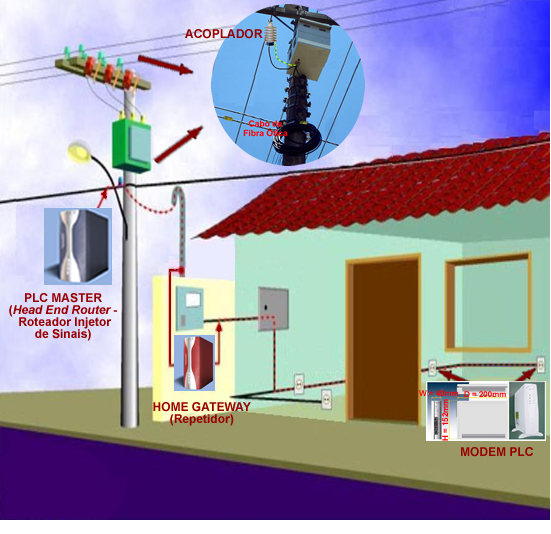
\includegraphics[width=0.8\textwidth]{arquitetura_plc.png}
    \caption{Arquitetura de uma rede Power Line Communication.}
    \label{fig:Figura}
\end{figure}

\section{Problemas na transmissão}

\subsection{Eco: O que é e Principais causas}
O eco é causado por descontinuidades na linha, como mudanças de impedância, criando interferência no sinal transmitido. Ocorre quando um sinal transmitido é refletido de volta para a fonte. Acontece geralmente por problemas físicos como conexões defeituosas ou terminais mal conectados. Esse eco cria interferência no sinal recebido, prejudicando a interpretação correta dos dados.

\begin{enumerate}
\item Impedância Mismatch: Diferenças na impedância entre o transmissor, a linha e o receptor, o que faz com que parte do sinal seja refletida de volta. Como Mencionado por \cite{wang2019} Em sistemas PLC, o casamento de impedância é geralmente alcançado por meio de uma rede de casamento de impedância (circuito). Um acoplador PLC normalmente inclui um circuito de acoplamento e um circuito de casamento de impedância, projetado para obter o casamento de impedância entre modems PLC e canais de linha de energia. Com isso em mente, vários fatores devem ser considerados ao projetar um circuito de casamento de impedância, como ganho e perda de inserção, eficiência e custo, largura de banda e atenuação, e região de casamento e estrutura.
\item Filtros Mal Configurados: Filtros de linha inadequados podem criar reflexões.
\item Ruídos e Interferência: Ruídos elétricos na linha (devido a motores, eletrodomésticos, etc.) podem amplificar ou causar ecos nos sinais.
\item Conexões Defeituosas: Conexões mal feitas ou oxidadas podem criar um "ponto de reflexão", que gera o eco.
\end{enumerate}

\subsection{Ruido: O que é e Principais causas}
Interferência gerada por dispositivos elétricos ou fontes externas, como motores, eletrodomésticos, ou fontes de radiação eletromagnética, que distorcem os sinais de comunicação. O ruído é um dos principais problemas que afetam a transmissão de dados em sistemas PLC, pois a rede elétrica não foi projetada originalmente para comunicação de dados. O ruído pode distorcer os sinais transmitidos, dificultando a recepção e a interpretação correta dos dados.
\begin{enumerate}
\item Equipamentos que usam a rede elétrica podem gerar interferência eletromagnética, como motores, fontes de alimentação comutadas (de computadores e carregadores de dispositivos), eletrodomésticos (geladeiras, micro-ondas, etc.), lâmpadas fluorescentes e dimmers. Esses dispositivos introduzem ruído de alta frequência na linha.

\item A Interferência Eletromagnética pode ser causada por fontes externas à rede elétrica, como sinais de rádio, antenas, torres de celular ou qualquer dispositivo que emita radiação eletromagnética. Como os sinais PLC operam em frequências semelhantes às utilizadas por muitos desses dispositivos, eles podem interferir nos sinais de comunicação.
\item Conexões ruins, fiação antiga ou mal feita, e componentes defeituosos podem introduzir ruído na rede, gerando problemas na comunicação.
\end{enumerate}

\subsection{Atenuação: O que é e Principais causas}
Atenucação é a perda gradual da intensidade do sinal à medida que ele se propaga pela rede elétrica, devido à resistência dos cabos, distância ou imperfeições na fiação.

\begin{enumerate}
\item A atenuação ocorre quando o sinal transmitido pela rede elétrica perde força à medida que se propaga pela linha. Essa perda de intensidade pode comprometer a qualidade da transmissão de dados.
\item Quanto maior a distância entre o transmissor e o receptor, maior será a perda de sinal, já que a energia do sinal se dissipa ao longo da fiação elétrica.
\item Fiação elétrica antiga, oxidada ou de má qualidade pode aumentar a resistência e, portanto, a atenuação do sinal. Além disso, a fiação inadequada pode amplificar as perdas.
\item Conexões mal feitas, cabos danificados e dispositivos conectados à rede podem criar pontos de perda de sinal, aumentando a atenuação.
\end{enumerate}

\section{Transmissões Paralelas}
A transmissão de dados paralela é uma técnica de comunicação na qual múltiplos bits são transmitidos simultaneamente através de vários canais de comunicação. Ao contrário da transmissão em série, onde os dados são enviados bit a bit por um único canal, a transmissão paralela utiliza vários fios ou condutores, permitindo que um número maior de bits seja enviado ao mesmo tempo. Isso resulta em uma maior taxa de transferência de dados em distâncias curtas.

Cada fio em uma transmissão paralela carrega um bit individual de informação, e todos os bits de um byte, por exemplo, podem ser enviados simultaneamente. O número de fios utilizados define quantos bits podem ser transmitidos ao mesmo tempo — por exemplo, uma interface paralela de 8 bits usa 8 fios para transmitir 8 bits de uma só vez.

\subsubsection{Vantagens:}
\begin{enumerate}
    \item Alta velocidade de transmissão: Como vários bits são enviados ao mesmo tempo, a transmissão paralela pode alcançar uma taxa de dados muito maior do que a transmissão em série em distâncias curtas.
    \item Sincronização simplificada: Quando o \textit{\textit{clock}} é compartilhado, a sincronização de múltiplos bits pode ser mais fácil, pois todos os bits chegam praticamente ao mesmo tempo, exigindo menos controle de sincronismo individual.
\end{enumerate}

\subsubsection{Desvantagens:}
\begin{enumerate}
    \item Custo elevado: A necessidade de vários condutores para transmitir os dados aumenta a complexidade e o custo do sistema, tanto em termos de cabos quanto de conectores.
    \item Problemas de distorção e interferência: Em transmissões paralelas de longa distância, a diferença no tempo de chegada dos bits, conhecida como skew, pode causar erros de transmissão. Além disso, a interferência entre os fios paralelos pode degradar o sinal, limitando a eficácia desse tipo de transmissão a curtas distâncias.
\end{enumerate}

\subsubsection{Aplicações}
\begin{enumerate}
    \item Porta Paralela (LPT): Muito utilizada em computadores antigos para conectar impressoras. A interface paralela da porta LPT permitia a transferência de 8 bits simultaneamente, acelerando a comunicação com dispositivos de impressão. \ref{fig:Figura2}



    \item Discos Rígidos com Interface PATA (Parallel ATA): Antes da adoção da interface SATA, muitos computadores utilizavam o padrão PATA (também conhecido como IDE). Essa interface permitia a transmissão paralela de dados, enviando vários bits ao mesmo tempo para aumentar a velocidade de transferência entre o disco rígido e o sistema.

    \item Barramentos PCI (Peripheral Component Interconnect): Barramentos PCI tradicionais utilizavam transmissão paralela para conectar dispositivos como placas de som, placas de rede e placas de vídeo em sistemas mais antigos. O PCI foi amplamente substituído pelo PCI Express, que usa transmissão em série. \ref{fig:Figura3}

    \item Barramentos de Dados Internos em CPUs: Em muitos sistemas computacionais, o barramento de dados que conecta a CPU à memória ou outros dispositivos periféricos usava ou ainda usa transmissão paralela para acelerar o fluxo de informações.

    \item Impressoras de Impacto e Matriciais: Além de impressoras modernas, impressoras antigas, especialmente impressoras de impacto e matriciais, também faziam uso de portas paralelas para transferir dados de forma mais eficiente.
\end{enumerate}

\begin{figure}[h]
    \centering
    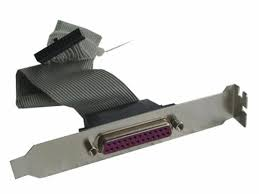
\includegraphics[width=0.5\textwidth]{lpt1_conector.jpeg}
    \caption{Cabo Conector Porta Paralela LPT1.}
    \label{fig:Figura2}
\end{figure}

\begin{figure}[h]
    \centering
    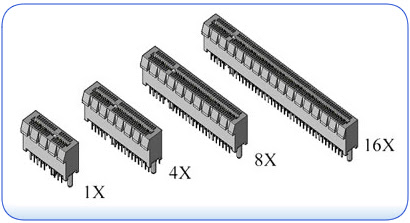
\includegraphics[width=0.7\textwidth]{barramentos_pci.jpg}
    \caption{Barramento de Interconexão de componentes periféricos.}
    \label{fig:Figura3}
\end{figure}
\section{Transmissões em Série Assíncronas e Síncronas}

A transmissão de dados em série é um método em que os dados são enviados bit a bit através de um único canal de comunicação. Esse processo contrasta com a transmissão paralela, na qual vários bits são transmitidos simultaneamente por canais diferentes. No entanto, dentro do escopo de transmissões em série, dois tipos principais são utilizados: transmissões assíncronas e síncronas. Cada um tem suas características próprias de operação, sincronização e aplicabilidade.


\subsection{Transmissão em Série Assíncrona}
Na transmissão em série assíncrona, não há um sinal de \textit{clock} compartilhado entre o transmissor e o receptor para manter a sincronização contínua dos dados. Em vez disso, a sincronização é feita a cada bloco de dados por meio de bits de início (start bits) e bits de parada (stop bits). Cada bloco de dados, geralmente composto de 8 bits, é precedido por um start bit e seguido por um ou mais stop bits. Quando o receptor detecta o start bit, ele usa seu próprio \textit{clock} interno para determinar o momento correto de ler os bits de dados. Após o último stop bit, o receptor aguarda o próximo start bit para retomar a comunicação.

\subsubsection{Características principais:}
\begin{enumerate}
\item Independência de \textit{clock} contínuo: The transmissor and the receptor operate independently of the \textit{clock}s.
\item Sincronização por bloco: A sincronização ocorre para cada bloco de dados, utilizando bits adicionais.
\item Aplicações comuns: Transmissões assíncronas são comumente utilizadas em interfaces seriais como RS-232 e UART, onde a simplicidade do protocolo é desejada, e a sobrecarga de bits de controle é tolerada.
\end{enumerate}

\subsubsection{Vantagens:}
\begin{enumerate}
    \item Menor complexidade, já que não há necessidade de manter \textit{clock}s sincronizados continuamente.
    \item Flexibilidade em sistemas que não requerem altas taxas de transmissão de dados.
\end{enumerate}

\subsubsection{Desvantagens:}
\begin{enumerate}
    \item Eficiência reduzida devido à sobrecarga de bits extras (start e stop) em cada transmissão.
    \item O erro de sincronização pode ocorrer se os \textit{clock}s do transmissor e receptor se desajustarem significativamente ao longo do tempo.
\end{enumerate}

\subsection{Transmissão Síncrona}
Na transmissão síncrona, o transmissor e o receptor compartilham o mesmo \textit{clock}, o que garante uma sincronização constante.Um \textit{clock} é enviado junto com os dados ou é previamente acordado entre os dispositivos. Isso permite que os dados sejam transmitidos de forma contínua, sem a necessidade de start/stop bits. O \textit{clock} comum mantém o sincronismo entre transmissor e receptor para que ambos saibam quando amostrar os dados.

\subsubsection{Vantagens:}
\begin{enumerate}
    \item Maior eficiência na transmissão: Em transmissões síncronas, não há a necessidade de bits de início (start) e parada (stop) para cada bloco de dados, o que permite um fluxo contínuo e mais rápido de informações. Isso resulta em um uso mais eficiente da largura de banda.
    
    \item Sincronização contínua: O compartilhamento de um \textit{clock} comum entre transmissor e receptor garante que ambos estejam sempre sincronizados, o que minimiza a possibilidade de erros na transmissão de dados devido à falta de sincronização.
\end{enumerate}

\subsubsection{Desvantagens:}
\begin{enumerate}
    \item Complexidade de implementação: A necessidade de manter um \textit{clock} compartilhado entre os dispositivos adiciona complexidade ao projeto de sistemas síncronos, tanto em termos de hardware quanto de software. Isso pode aumentar o custo e a dificuldade de implementação.
    
    \item Sensibilidade à distância: Como o \textit{clock} precisa ser compartilhado entre transmissor e receptor, transmissões síncronas podem ser menos confiáveis em longas distâncias, onde a degradação do sinal do \textit{clock} pode afetar a precisão da sincronização.
\end{enumerate}

\subsection{\textit{clock} (Temporizador ou Relógio)}
Os \textit{clock}s em sistemas digitais operam como um trem de pulsos de período T chamado de \textit{clock} (relógio ou temporizador), a cada transição de \textit{clock} dizemos que a máquina passa para um próximo estado, entre níveis alto e baixo. Esses pulsos determinam quando os dispositivos devem ler ou escrever dados, garantindo que todos os componentes envolvidos na transmissão estejam "no mesmo ritmo". A frequência do \textit{clock} é o número de ciclos completos (de nível alto para baixo e de volta ao alto) por segundo, medida em hertz (Hz). Por exemplo, um \textit{clock} de 1 MHz (1 milhão de hertz) tem 1 milhão de pulsos por segundo. Em resumo, o \textit{clock} é um sinal de referência que sincroniza a troca de dados entre diferentes partes de um sistema, essencial em sistemas síncronos, mas também usado indiretamente em sistemas assíncronos para garantir que os dispositivos estejam alinhados.

\section{Multiplexação}
É uma técnica usada em telecomunicações e redes de computadores para transmitir múltiplos sinais ou fluxos de dados simultaneamente por um único canal de comunicação. O objetivo principal da multiplexação é otimizar o uso da largura de banda, permitindo que várias comunicações compartilhem o mesmo meio físico sem interferir entre si. Existem diferentes tipos de multiplexação, dependendo de como os sinais são organizados e transmitidos. \ref{fig:Figura4} 

\subsection{FDM (Frequency Division Multiplexing)}
A multiplexação por divisão de frequência (FDM) divide a largura de banda total de um canal em várias subfaixas de frequência, cada uma dedicada a uma comunicação separada. Cada sinal de dados é modulado em uma portadora de frequência diferente, e todos os sinais são transmitidos ao mesmo tempo, mas em diferentes faixas de frequência. Um exemplo clássico de FDM é o rádio FM, onde cada estação transmite em uma frequência diferente, mas todos os sinais estão compartilhando o mesmo espectro. Dentre as aplicações mais comuns temos: Rádio, televisão por cabo, sistemas de comunicação por satélite. \ref{fig:Figura5} \cite{pinto_albuquerque}

\subsection{TDM (Time Division Multiplexing)}
A multiplexação por divisão de tempo (TDM) divide o tempo em slots ou intervalos, e cada sinal de dados é transmitido em um intervalo de tempo específico. Em TDM, os sinais compartilham o mesmo canal físico, mas cada sinal usa o canal por um curto período de tempo, de forma sequencial. Isso ocorre em ciclos, em que cada sinal tem a oportunidade de transmitir seus dados durante o seu intervalo de tempo. Um exemplo de TDM é o sistema de telefonia digital. Dentre as aplicações mais comuns temos telefonia digital, redes SONET/SDH. \ref{fig:Figura6} \cite{promader2015}

\begin{figure}[H]
    \centering
    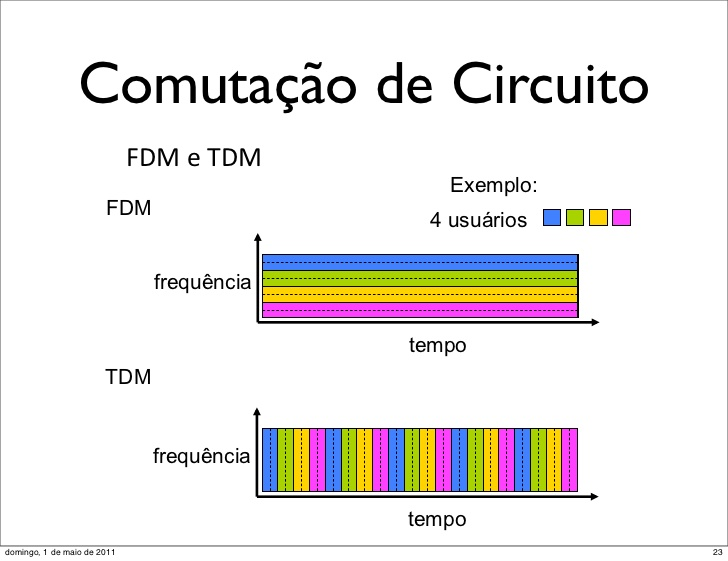
\includegraphics[width=0.7\textwidth]{tdm_fdm.jpg}
    \caption{Comutação de circuito FDM x TDM.}
    \label{fig:Figura4}
\end{figure}

\begin{figure}[H]
    \centering
    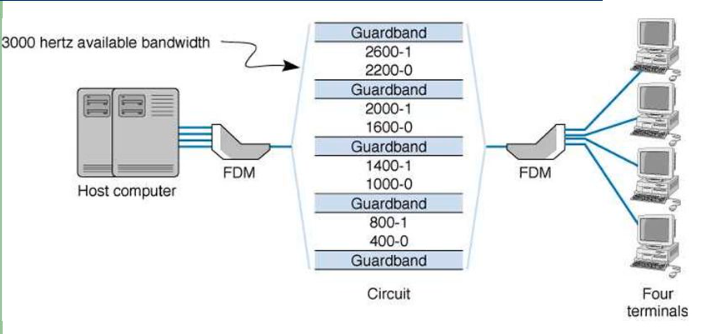
\includegraphics[width=0.7\textwidth]{FDM2.png}
    \caption{Exemplo de FDM.}
    \label{fig:Figura5}
\end{figure}

\begin{figure}[H]
    \centering
    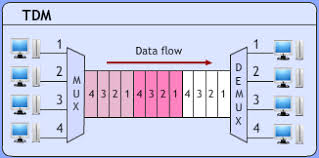
\includegraphics[width=0.7\linewidth]{TDM-example.jpeg}
    \caption{Exemplo de TDM.}
    \label{fig:Figura6}
\end{figure}

\section{Canais de Comunicação e Modos de Operação de Comunicação}
Os canais de comunicação se referem aos meios pelos quais as informações são transmitidas entre dois ou mais pontos (como dispositivos ou sistemas). Eles podem ser físicos, como cabos, ou sem fio, como sinais de rádio. Esses canais têm diferentes modos de operação, que determinam como a comunicação ocorre, especificamente como os dados fluem entre as partes envolvidas. \cite{galvao2024}

\begin{figure}[H]
    \centering
    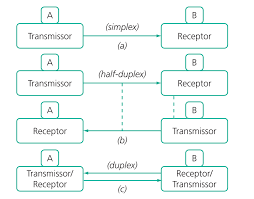
\includegraphics[width=0.5\linewidth]{modos_com_2.png}
    \caption{Modos de Operação de Comunicação.}
    \label{fig:Figura7}
\end{figure}

\subsubsection{Simplex}
A comunicação é essencialmente unidirecional, ou seja, os dados só fluem em uma direção. Imagine um cenário em que um computador envia constantemente dados para um monitor. O monitor apenas recebe os dados que são transmitidos pela máquina e nunca envia informações de volta. Esse fluxo unidirecional é característico do simplex: o transmissor envia informações sem esperar uma resposta, e o receptor apenas recebe os dados passivamente. O rádio tradicional é um exemplo clássico de simplex, onde a estação de rádio envia sinais que os rádios domésticos recebem, mas os rádios não têm como responder ou enviar dados de volta à estação. A simplicidade desse modelo é uma vantagem em situações onde a comunicação de retorno não é necessária, mas a principal limitação é a falta de interatividade, já que não há como o receptor enviar informações de volta ao transmissor. \cite{galvao2024}

\subsubsection{Half-Duplex}
Aqui as coisas se tornam um pouco mais interativas, mas com uma restrição importante: os dispositivos podem se comunicar em ambas as direções, porém não ao mesmo tempo. Pense em um walkie-talkie: quando uma pessoa fala, o outro aparelho só pode escutar, e enquanto essa pessoa fala, o receptor deve esperar sua vez de responder. Quando o primeiro dispositivo termina de falar, ele pode se tornar receptor, e o outro transmissor. Essa troca entre transmitir e receber é uma característica chave do half-duplex. É eficiente em contextos onde a comunicação bidirecional é necessária, mas não precisa acontecer simultaneamente. No entanto, a alternância entre transmitir e receber pode causar atrasos e diminui a eficiência quando há necessidade de muita troca de dados rapidamente, como em sistemas de redes de computadores que precisam esperar a vez de enviar ou receber. \cite{galvao2024}

\subsubsection{Full-Duplex}
No modo full-duplex, a comunicação é totalmente fluida, ocorrendo em ambas as direções ao mesmo tempo. Em uma chamada telefônica, por exemplo, tanto você quanto a pessoa do outro lado podem falar e escutar simultaneamente. Não há necessidade de esperar para falar ou para ouvir, pois o canal de comunicação é aberto para as duas direções ao mesmo tempo. Nos sistemas modernos de rede de computadores, como em conexões Ethernet, full-duplex permite que os dispositivos enviem e recebam dados simultaneamente, o que resulta em uma comunicação muito mais rápida e eficiente. Isso ocorre porque o canal de comunicação é dividido de forma que a transmissão e a recepção de dados aconteçam simultaneamente, eliminando o tempo de espera que seria necessário no half-duplex. Esse modelo é ideal para sistemas que precisam de comunicação constante e de alto desempenho, como na transmissão de grandes volumes de dados ou em cenários que exigem interações em tempo real. \cite{galvao2024}

\subsection{Modos de Operação em Power Line Communication}
A Tabela~\ref{tab:modos-comunicacao} apresenta exemplos práticos de cada modo de operação aplicado a sistemas PLC.

\begin{table}[h!]
\centering
\caption{Modos de Operação em PLC}
\label{tab:modos-comunicacao}
\begin{tabular}{|c|p{4cm}|p{8cm}|}
\hline
\textbf{Modo}     & \textbf{Descrição}                                                                                         & \textbf{Exemplo de Aplicação}                                                                                                                                                                                                 \\ \hline
\textit{Simplex}  & Comunicação unidirecional.                                                                                 & Um medidor de energia envia dados de consumo à central de monitoramento, sem necessidade de resposta.                                                                                                                           \\ \hline
\textit{Half-duplex} & Comunicação bidirecional alternada.                                                                      & Sensores de movimento enviam informações ao controlador de iluminação, e este responde com comandos de ativação/desativação das luzes, porém não ao mesmo tempo.                                                               \\ \hline
\textit{Full-duplex} & Comunicação bidirecional simultânea.                                                                     & Redes PLC domésticas que utilizam adaptadores Powerline para transmitir internet, permitindo a comunicação simultânea em ambas as direções, como em streaming de vídeos e jogos online.                                          \\ \hline
\end{tabular}
\end{table}

\noindent Os modos \textit{half-duplex} e \textit{full-duplex} são amplamente utilizados em redes de automação e comunicação doméstica, dependendo das necessidades de velocidade e simultaneidade da troca de informações.

\section{Conclusão}

A pesquisa realizada proporcionou \textit{insights} valiosos sobre os temas e problemas abordados, explorando uma tecnologia fundamental na história da \textit{comunicação de dados}, a \textit{Power Line Communication (PLC)}.

Os resultados apresentados elucidaram as principais vantagens e desvantagens dos tópicos discutidos. A metodologia adotada foi eficaz ao abordar de maneira abrangente problemas comuns a diferentes formas de comunicação de dados, enquanto focou em aspectos específicos das PLCs, oferecendo uma análise detalhada sobre suas aplicações e desafios.

Para futuros trabalhos, recomenda-se um aprofundamento nas áreas de \textit{Engenharia Elétrica}, com o objetivo de realizar experimentos práticos mais robustos no contexto de PLC. Além disso, o estudo das \textit{redes de computadores} pode oferecer novas perspectivas e otimizações no uso dessa tecnologia.


\bibliographystyle{sbc}
\bibliography{sbc-template}

\end{document}
